\textbf{\LARGE osn 21. Базы данных. Основные понятия реляционной модели данных. Реляционная алгебра. Средства языка запросов SQL.}


\textbf{Основные понятия реляционной модели данных:}

\begin{itemize}
    \item Понятие \textbf{типа данных} в реляционной модели данных полностью соответствует понятию типа данных в языках программирования, состоит из трех основных компонентов: определение множества значений данного типа; определение набора операций, применимых к значениям типа; определение способа внешнего представления значений типа (литералов).
    \item \textbf{Домен} --- допустимое потенциальное, ограниченное подмножество значений данного типа.
    \item Для уточнения термина отношение выделяются понятия заголовка отношения, значения отношения и переменной отношения.
    Пусть дана совокупность типов данных $T_1, T_2, \dots, T_n$, называемых также доменами, не обязательно различных. Тогда $n$-арным \textbf{отношением} $R$, или отношением $R$ степени $n$ называют подмножество декартовa произведения множеств $T_1, T_2, \dots, T_n$.
    \item \textbf{Тело отношения} -- это множество кортежей вида $\{<A_1, T_1, v_1>, < A_2, T_2, v_2 >,\dots, < A_n, T_n, v_n>\}$, где $v_i \in T_i$, $A_i$ -- столбцы (атрибуты) отношения. 

\end{itemize}

\textbf{Алгебра Кодда -- основные реляционные операции}
\begin{itemize}
    \item При выполнении операции \textbf{объединения} (\textit{UNION}) двух отношений производится отношение, включающее все кортежи, входящие хотя бы в одно из отношений-операндов.
    \item Операция \textbf{пересечения} (\textit{INTERSECT}) двух отношений производит отношение, включающее все кортежи, входящие в оба отношения-операнда.
    \item Отношение, являющееся \textbf{разностью} (\textit{MINUS}) двух отношений, включает все кортежи, входящие в отношение-первый операнд, такие, что ни один из них не входит в отношение, являющееся вторым операндом.
    \item При выполнении \textbf{декартова произведения} (\textit{TIMES}) двух отношений производится отношение, кортежи которого являются конкатенацией (сцеплением) кортежей первого и второго операндов.
    \item Результатом \textbf{ограничения} (\textit{WHERE}) отношения по некоторому условию является отношение, включающее кортежи отношения-операнда, удовлетворяющее этому условию.
    \item При выполнении \textbf{проекции} (\textit{PROJECT}) отношения на заданное подмножество множества его атрибутов производится отношение, кортежи которого производятся путем взятия соответствующих значений из кортежей отношения-операнда.
    \item При \textbf{соединении} (\textit{JOIN}) двух отношений по некоторому условию образуется результирующее отношение, кортежи которого являются конкатенацией кортежей первого и второго отношений и удовлетворяют этому условию.
    \item У операции \textbf{реляционного деления} (\textit{DIVIDE BY}) два операнда – бинарное и унарное отношения. Результирующее отношение состоит из унарных кортежей, включающих значения первого атрибута кортежей первого операнда таких, что множество значений второго атрибута (при фиксированном значении первого атрибута) включает множество значений второго операнда.
    \item Операция \textbf{переименования} (\textit{RENAME}) производит отношение, тело которого совпадает с телом операнда, но имена атрибутов могут быть изменены.
    \item Операция \textbf{присваивания} (\textit{:=}) позволяет сохранить результат вычисления реляционного выражения в существующем отношении БД.
\end{itemize}

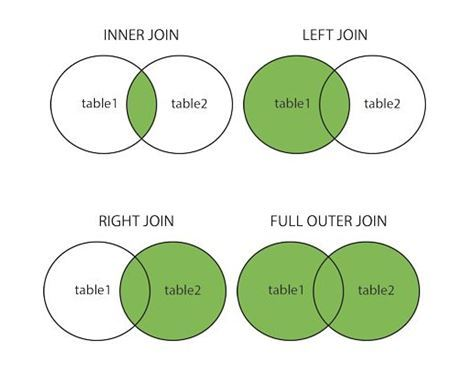
\includegraphics[width=\columnwidth]{pics/osn21_join.jpg}

\textbf{Алгебра Кодда -- специальные реляционные операции}

Имеются важные частные случаи соединения – \textbf{эквисоединение} (\textit{EQUIJOIN}) и \textbf{естественное соединение} (\textit{NATURAL JOIN}).
\begin{itemize}
    \item Операция соединения называется операцией \textbf{эквисоединения}, если условие соединения имеет вид (a = b), где a и b – атрибуты разных операндов соединения.
    \item Пусть AB обозначает объединение заголовков отношений A и B. Тогда \textbf{естественное соединение} A и B – это спроецированный на AB результат эквисоединения A и B по условию A.c = B.c.
\end{itemize}

\textbf{Язык SQL}

\textbf{SQL} --- универсальный компьютерный язык, применяемый для создания, модификации и управления данными в реляционных базах данных.
SQL основывается на реляционной алгебре. Язык SQL представляет собой совокупность операторов, инструкций и вычисляемых функций. Операторы SQL делятся на:
\begin{enumerate}
    \item \textbf{операторы определения данных} (Data Definition Language, DDL):
    \begin{itemize}
        \item[--] \textit{CREATE} создает объект БД (саму базу, таблицу, представление, пользователя и т. д.);
        \item[--] \textit{ALTER} изменяет объект;
        \item[--] \textit{DROP} удаляет объект.
    \end{itemize}
    \item \textbf{операторы манипуляции данными} (Data Manipulation Language, DML):
    \begin{itemize}
        \item[--] \textit{SELECT} считывает данные, удовлетворяющие условиям;
        \item[--] \textit{INSERT} добавляет новые данные;
        \item[--] \textit{UPDATE} изменяет существующие данные;
        \item[--] \textit{DELETE} удаляет данные.
    \end{itemize}
    \item \textbf{операторы определения доступа к данным} (Data Control Language, DCL):
    \begin{itemize}
        \item[--] \textit{GRANT} предоставляет пользователю (группе) разрешения на определенные операции с объектом;
        \item[--] \textit{REVOKE} отзывает ранее выданные разрешения;
        \item[--] \textit{DENY} задает запрет, имеющий приоритет над разрешением.
    \end{itemize}
    \item \textbf{операторы управления транзакциями} (Transaction Control Language, TCL):
    \begin{itemize}
        \item[--] \textit{COMMIT} применяет транзакцию;
        \item[--] \textit{ROLLBACK} откатывает все изменения, сделанные в контексте текущей транзакции;
        \item[--] \textit{SAVEPOINT} делит транзакцию на более мелкие участки.
    \end{itemize}
\end{enumerate}

\textbf{Пример:} Выбрать среднюю зарплату продавцов, которые обслуживают покупателей их штата 'CA'.
\begin{lstlisting}[language=SQL]
    SELECT employee.last_name, employee.salary FROM 
    employee JOIN job using (job_id)
    JOIN customer ON employee_id = salesperson_id 
    WHERE customer.state = 'CA' AND 
    job.function = 'SALESPERSON';
\end{lstlisting}


% -------- source --------
\bigbreak
[\cite{bdbook}]